\chapter{Heisenbergsche Unsch"arferelation\label{chapter:heisenberg}}
\lhead{Heisenbergsche Unsch"arferelation}
\rhead{}

In der Quantenmechanik lassen sich die Observablen nicht mehr einfach
vertauschen, wie das in der klassischen Mechanik m"oglich war.
F"ur Operatoren gilt im Allgemeinen kein Kommutativgesetz.
In diesem Abschnitt wollen wir die Konsequenzen dieser Tatsache
untersuchen.
Wir k"onnen aber bereits jetzt feststellen, dass die Gleichung
$AB=BA$ f"ur zwei quantenmechanische Observable ``fast'' stimmen
muss, in dem Sinne, dass der Unterschied der beiden Seiten sehr
klein sein muss. 

\section{Vertauschungsrelationen und Eigenvektoren}
\rhead{Vertauschungsrelationen und Eigenvektoren}
%\subsection{Definitionen}
\index{Kommutator}
\index{Antikommutator}
Zu zwei Operatoren $A$ und $B$ kann man Kommutator und Antikommutator
bilden:
\[
\begin{aligned}
&\text{Kommutator:}&
[A,B]&=AB-BA
\\
&\text{Antikommutator:}&
\{A,B\}&=AB+BA
\end{aligned}
\]
Wenn $[A,B]=AB-BA=0$ folgt $AB=BA$,
der Kommutator gibt also an, ob die beiden Operatoren vertauschen (kommutieren).
Wenn $\{A,B\}=AB+BA=0$ folgt $AB=-BA$,
der Kommutator gibt also an, ob die beiden Operatoren antikommutieren.

\subsection{Kommutator und Eigenvektoren}
Falls $A$ and $B$ Observable sind, die nicht vertauschen, dann k"onnen
gemeinsame Eigenvektoren nicht beliebig sein.

\begin{hilfssatz}
\label{skript:kommutatorannihliertev}
Der Kommutator $[A,B]$ annihiliert gemeinsame Eigenvektoren von $A$ und $B$.
\end{hilfssatz}

\begin{proof}[Beweis]
Nehmen wir an, $|\psi\rangle$ sei ein gemeinsamer Eigenvektor
von $A$ mit Eigenwert $\alpha$ und $B$ mit Eigenwert $\beta$.
Dann wirkt der Kommutator auf $|\psi\rangle$ wie folgt
\[
[A,B]\,|\psi\rangle
=
(AB-BA)\,|\psi\rangle 
=
A\beta\,|\psi\rangle -B\alpha\,|\psi\rangle
=
\alpha\beta\,|\psi\rangle-\beta\alpha\,|\psi\rangle
=
0.
\]
Ein gemeinsamer Eigenvektor $|\psi\rangle$ wird also von $[A,B]$
zu $0$ gemacht.
\end{proof}

In vielen F"allen ist der Kommutator ein Vielfaches der identischen
Abbildung. F"ur diese F"alle l"asst sich eine etwas sch"arfere
Folgerung ableiten.

\begin{satz}
Wenn zwei Observable einen Kommutator haben, der ein Vielfaches
der identischen Abbildung ist, dann haben die Observable keine
gemeinsamen Eigenvektoren.
\end{satz}

\begin{beispiel}
F"ur die Observablen $X$ f"ur Ort und $P$ f"ur den Impuls eines Teilchens,
k"onnen wir den Kommutator in der Ortsdarstellung explizt ausrechnen:
\begin{align*}
[X,P]\psi(x)
&=
\biggl[
x,\frac{\hbar}{i}\frac{\partial}{\partial x}
\biggr]\psi(x)
=
x\frac{\hbar}{i}\frac{\partial\psi(x)}{\partial x}
-
\frac{\hbar}{i}\frac{\partial}{\partial x}\bigl(x\psi(x)\bigr)
\\
&=
x\frac{\hbar}{i}\frac{\partial\psi(x)}{\partial x}
-
\frac{\hbar}{i}\psi(x)
-
\frac{\hbar}{i}x\frac{\partial\psi(x)}{\partial x}
=
-\frac{\hbar}{i}\psi(x).
\end{align*}
Der Kommutator ist also
\[
[X,P]=-\frac{\hbar}{i}\operatorname{id},
\]
ein Vielfaches der identischen Abbildung.
Die identische Abbildung hat nat"urlich keine Vektoren, die von ihr
annihiliert werden.
Orts- und Impuls-Operatoren k"onnen also keine gemeinsamen Eigenvektoren
haben.
\end{beispiel}

\subsection{Eigenbasen von zwei Operatoren}
Umgekehrt stellt sich die Frage, unter welchen Voraussetzungen zwei
Observable eine Basis von gemeinsamen Eigenvektoren haben k"onnen.
Der n"achste Satz liefert ein Kriterium daf"ur.

\begin{satz}
\label{skript:kommevbasis}
Wenn zwei selbstadjungierte Operatoren vertauschen, dann gibt es eine
gemeinsame Basis von Eigenvektoren.
\end{satz}

\begin{proof}[Beweis]
Wir f"uhren den Beweis nur f"ur einen endlichdimensionalen Zustandsraum.
Seien also $A$ und $B$ zwei selbstadjungierte Operatoren mit $[A,B]=0$.
Ist $v$ ein Eigenvektor von $A$ zum Eigenwert $a$, dann gilt
$ Av=av $.
F"ur den Vektor $Bv$ gilt dann
\[
A(Bv)=BAv=Bav=aBv,
\]
$Bv$ ist also ebenfalls ein Eigenvektor von $A$ zum gleichen Eigenwert.
F"ur einen Eigenvektor $u$ von $B$ gilt analog, dass $Au$ ein Eigenvektor
von $B$ zum gleichen Eigenwert ist.

Zu jedem Eigenwert $a$ von $A$ sie $E_a$ der Raum der von den 
Eigenvektoren von $A$ zum Eigenwert $a$ aufgespannte Vektorraum.
$E_a$ heisst Eigenraum von $A$ zum Eigenwert $a$.
Nach Satz~\ref{skript:evorthogonal} sind die Eigenr"aume $E_a$ 
f"ur verschiedene $a$ orthogonal, und in jedem Eigenraum wirkt $A$
wie das $a$-fache der Einheitsmatrix.

Es gibt nur endliche viele verschiedene Eigenwert $a_1,\dots,a_k$.
Bildet man eine Basis des Zustandsraumes, indem man in jedem $E_{a_i}$
eine Basis w"ahlt, dann bekommt $A$ die Form
\[
A=\left(
\begin{array}{ccccccccccc}
a_1   &\dots &0     &      &      &      &      &      &      &      &      \\
\vdots&\ddots&\vdots&      &      &      &      &      &      &      &      \\
0     &\dots &a_1   &      &      &      &      &      &      &      &      \\
%\hline
      &      &      &a_2   &\dots &0     &      &      &      &      &      \\
      &      &      &\vdots&\ddots&\vdots&      &      &      &      &      \\
      &      &      &0     &\dots &a_2   &      &      &      &      &      \\
%\hline
      &      &      &      &      &      &\ddots&      &      &      &      \\
      &      &      &      &      &      &      &\ddots&      &      &      \\
%\hline
      &      &      &      &      &      &      &      &a_k   &\dots &0     \\
      &      &      &      &      &      &      &      &\vdots&\ddots&\vdots\\
      &      &      &      &      &      &      &      &0     &\dots &a_k   
\end{array}
\right)
\]

Weiter oben wurde gezeigt, dass der Operator $B$ die Eigenr"aume $E_a$ in sich
abbildet: $BE_a\subset E_a$. Da $B$ ausserdem selbstadjungiert ist, kann man
in jedem Eigenraum $E_{a_i}$ eine Basis
${\cal B}_i= \{b_1^{(i)},\dots,b_{l_i}^{(i)}\}$
aus Eigenvektoren f"ur $B$ finden. Die Vektoren $b_j^{(i)}$ sind nach
Konstruktion sowohl Eigenvektoren von $A$ zum Eigenwert $a_i$ als auch
Eigenvektoren von $B$. Die Vereinigung
\[
{\cal B}
=
\bigcup_{i=1}^k{\cal B}_i
=
\{
b_1^{(1)},\dots,b_{l_1}^{(1)},
b_1^{(2)},\dots,b_{l_2}^{(2)},
\dots,
b_k^{(k)},\dots,b_{l_k}^{(k)}
\}
\]
der Basen ${\cal B}_i$ ist eine Basis des Zustandsraumes aus gemeinsamen
Eigenvektoren von $A$ und $B$, in ihr haben beide Operatoren Diagonalform.
\end{proof}

\begin{satz}
Zwei Observablen haben genau dann eine gemeinsame Basis aus Eigenvektoren,
wenn sie vertauschen.
\end{satz}

\begin{proof}[Beweis]
Aus Satz~\ref{skript:kommevbasis} leiten wir ab, dass das Kriterium
gen"ugend ist.
Der Kommutator $[A,B]$ annihiliert gemeinsame Eigenvektoren von $A$
und $B$.
G"abe es eine Basis aus Eigenvektoren, dann m"usste der Kommutator alle
Basisvektoren annihilieren, es folgte $[A,B]=0$. Dieser
Widerspruch zeigt, dass das Kriterium auch notwendig ist.
\end{proof}


\section{Unscharfe Kenntnis von Observablen}
\rhead{Unscharfe Kenntnis von Observablen}
Im Allgemeinen kann man nicht annehmen, dass ein Beobachtung einer
Observablen $A$ im Zustand $|\psi\rangle$ immer den gleichen Wert ergibt.
Die Messwerte werden zum Beispiel wegen der unvermeidlichen
Unzul"anglichkeiten der Messung streuen.
Dann ist der Erwartungswert $\langle \psi|\,A\,|\psi\rangle$
der Observablen $A$ im Zustand $|\psi\rangle$ die genaueste Information,
die wir erhalten k"onnen.
Zur Abk"urzung schreiben wir $\langle A\rangle=\langle\psi|\,A\,|\psi\rangle$.
Mit $A$ ist auch $A-\langle A\rangle$ eine Observable, und ihr Erwartungswert
ist nat"urlich $0$.

Damit stellt sich die Frage, ob man f"ur spezielle Zust"ande eventuell
mehr Information erhalten kann.
Da die Varianz misst, wie stark die m"oglichen Werte streuen, suchen
wir Zust"ande mit verschwindender Varianz.
Es wird sich zeigen, dass dies genau die Eigenzust"ande sind.
Genaue Kenntnis von Observablenwerten ist also genau f"ur die
Eigenzust"ande m"oglich.

\subsection{Varianz}
In der Wahrscheinlichkeitsrechnung lernt man mit der Varianz eine
Gr"osse kennen, die angibt, wie nahe bei $\langle A\rangle$ die
Werte der Observable im Mittel anzutreffen sind.
Die Varianz ist die mittlere quadratische Abweichung, also der
Erwartungswert der Gr"osse $(A-\langle A\rangle)^2$, die auch wieder
eine Observable ist. Sie kann also mit unserem Formalismus berechnet
werden:
\begin{align*}
\operatorname{var}(A)
&=
\operatorname{var}_{|\psi\rangle}(A)
=
\langle \psi|\, (A-\langle A\rangle)^2\,|\psi\rangle
=
\langle\psi|\, A^2-2\langle A\rangle A+\langle A\rangle^2\,|\psi\rangle
\\
&=
\langle\psi|\,A^2\,|\psi\rangle 
-2\langle A\rangle \langle\psi|\,A\,|\psi\rangle
+\langle A\rangle^2\langle\psi|\psi\rangle
=\langle A^2\rangle -\langle A\rangle^2.
\end{align*}
Wir schreiben den Zustand als Index zum $\operatorname{var}$-Operator
nur, wenn nicht klar ist, welcher Zustand gemeint ist.
Dies entspricht der aus der Wahrscheinlichkeitsrechung bekannten Formel
$E(X^2)-E(X)^2$.
Wir nennen die Standardabweichung, also
\[
\sqrt{\operatorname{var}(A)}
=
\sqrt{\langle (A-\langle A\rangle)^2\rangle}
=
\sqrt{\langle A^2\rangle - \langle A\rangle^2}
\]
auch die {\em Unsch"arfe} der Messung von $A$, und schreiben daf"ur abgek"urzt
auch $\Delta A$.

Die Varianz misst, wie scharf ein Messwert in einem bestimmten Zustand
bekannt sein kann.
Der n"achste Satz zeigt, dass Zust"ande verschwindender Varianz
automatisch Eigenzust"ande sind. 
Von einem scharf definierten Wert einer Observablen kann man also nur
bei Eigenzust"anden sprechen.

\begin{satz}
Ist $A$ eine Observable und $|\psi\rangle$ ein Zustand, dann verschwindet
die Varianz im Zustand $|\psi\rangle$ genau dann, wenn $|\psi\rangle$
ein Eigenverktor von $A$ ist.
\end{satz}

\begin{proof}[Beweis]
Wir d"urfen ohne Einschr"ankung der Allgemeinheit annehmen, dass
$\langle\psi|\psi\rangle=1$. Ausserdem k"onnen wir schreiben
\[
A\,|\psi\rangle = a_{\|}\,|\psi\rangle + a_{\perp}\,|\varphi\rangle,
\]
wobei $|\varphi\rangle$ ein auf $|\psi\rangle$ senkrecht stehender,
normierter Vektor ist. Es ist also $\langle\psi|\varphi\rangle=0$
und $\langle\varphi|\varphi\rangle=1$.

Nach diesen Voraussetzungen berechnen wir jetzt die Varianz von $A$ im
Zustand $|\psi\rangle$:
\begin{align*}
\langle A\rangle
&=
\langle\psi|\,A\,|\psi\rangle
=
\langle\psi|\,a_{\|}\,|\psi\rangle
+
\langle\psi|\,b_{\perp}\,|\varphi\rangle
=
a_{\|}\langle\psi|\psi\rangle
+
b_{\perp}\langle\psi|\varphi\rangle
=
a_{\|}
\\
\langle A^2\rangle
&=
\langle\psi|\,A^2\,|\psi\rangle
=
(\langle\psi|\,\bar a + \langle\varphi|\,\bar a_{\perp})(a\,|\psi\rangle+a_{\perp}\,|\varphi\rangle)
\\
&=
\langle\psi|    \bar a_{\|} a_{\|} |\psi\rangle
+
\langle\psi|    \bar a_{\|} a_{\perp} |\varphi\rangle
+
\langle\varphi| \bar a_{\perp} a_{\|} |\psi\rangle
+
\langle\varphi| \bar a_{\perp} a_{\perp} |\varphi\rangle
\\
&=
|a_{\|}|^2+|a_{\perp}|^2
\\
\operatorname{var}(A)
&=
\langle A^2\rangle -\langle A\rangle^2
=
|a_{\|}|^2+|a_{\perp}|^2
-
a_{\|}^2
\end{align*}
Aus der Gleichung f"ur $\langle A\rangle$ kann man ablesen, dass $a_{\|}$ 
als Erwartungswert eines selbstadjungierten Operators reell ist.
Zusammen mit der Gleichung f"ur $\operatorname{var}(A)$ folgt daraus, dass
$
\operatorname{var}(A)=|a_{\perp}|^2
$ ist.

Wenn die Varianz verschwindet, dann muss also $a_{\perp}=0$ sein, somit
gilt f"ur $|\psi\rangle$, dass
\[
A\,|\psi\rangle = a_{\|}\,|\psi\rangle,
\]
$|\psi\rangle$ ist also ein Eigenvektor von $A$ zum Eigenwert $a_{\|}$.
Ist umgekehrt $|\psi\rangle$ ein Eigenvektor, dann ist $a_{\perp}=0$,
und die Varianz verschwindet.
\end{proof}

\subsection{Gleichzeitige Kenntnis von Observablen}
Exakte Kenntnis von Observablenwerten ist also genau dann m"oglich, wenn
ein Eigenzustand vorliegt.
Exakte Kenntnis der Werte von zwei Observablen $A$ und $B$ ist genau
dann m"oglich, wenn der Zustand ein Eigenzustand von {\em beiden }
Operatoren ist.
Vollst"andige gleichzeitige Kenntnis der Werte von zwei Observablen
ist also m"oglich, wenn es eine Basis des Zustandsraumes gibt, 
die aus Eigenvektoren f"ur beide Operatoren besteht. 
Mit Satz~\ref{skript:kommevbasis} k"onnen wir jetzt ein Kriterium
daf"ur formulieren:

\begin{satz} Gleichzeitige exakte Kenntnis von Observablen ist genau
m"oglich, wenn die Observablen vertauschen.
\end{satz}

In der klassischen Mechanik haben wir keine Schwierigkeit, Ort und
Impuls gleichzeitig festzustellen. Das liegt nat"urlich daran, dass
der Kommutator den sehr kleinen Faktor $\hbar$ enth"alt.
F"ur makroskopische Zwecke sind Ort und Impuls also gleichzeitig 
feststellbar.

%Wenn es also nicht m"oglich ist, Ort und Impuls eines Teilchens
%gleichzeitig exakt zu wissen, wie genau ist es dann m"oglich,
%Ort und Impuls zu wissen?
%Um diese Frage zu beantworten m"ussen wir zun"achst ein Mass f"ur
%die Genauigkeit finden, mit der Ort oder Impuls in einem bestimmten
%Zustand bekannt sein kann.
%Wir werden es die Unsch"arfe nennen.
%Wir erwarten dann eine Ungleichung, die uns sagt, wie grosse 
%Unsch"arfe sein muss, eine Unsch"arferelation.

\subsection{Kovarianz und Unsch"arfeprodukt}
Die Varianz ist ein Spezialfall der Kovarianz, die als 
\[
\operatorname{cov}(X,Y)
=
E((X-E(X))(Y-E(Y)))
\]
definiert war, $\operatorname{var}(X)=\operatorname{cov}(X,X)$.
Analog k"onnen wir jetzt auch eine Kovarianz f"ur Observable als
\[
\langle A,B\rangle
=
\langle\psi|
\,
(A-\langle A\rangle)(B-\langle B\rangle)
\,
|\psi\rangle
\]
definieren.
Man beachte, dass die Gr"osse $\langle A,B\rangle$ nicht symmetrisch zu
sein braucht, ausser wenn die Operatoren $A$ und $B$ vertauscht werden
k"onnen.


Man kann $\langle A,B\rangle$ auch als den Wert der Transformationsfunktion 
zweier Zust"ande ansehen:
\begin{equation}
\left.
\begin{aligned}
|a\rangle &= (A-\langle A\rangle)\,|\psi\rangle\\
|b\rangle &= (B-\langle B\rangle)\,|\psi\rangle
\end{aligned}
\right\}
\quad
\Rightarrow
\quad
\langle A,B\rangle = \langle a|b\rangle.
\end{equation}
Nat"urlich gilt die Cauchy-Schwarz-Ungleichung f"ur die beiden
Zust"ande $|a\rangle$ und $|b\rangle$, also
\begin{equation}
|\langle a|b\rangle|^2
\le
\langle a|a\rangle \langle b|b\rangle
=
\operatorname{var}(A)\operatorname{var}(B)
=\Delta A^2 \cdot \Delta B^2
\label{skript:cauchy-schwarz-uncertainty}
\end{equation}
Falls also die linke Seite nicht $0$ ist, dann k"onnen wir die beiden
Gr"ossen $A$ und $B$ nicht beliebig genau kennen.
Die Ungenauigkeit, mit der $A$ und $B$ bekannt sein k"onnen, sind "uber
die Ungleichung (\ref{skript:cauchy-schwarz-uncertainty}) miteinander verkn"upft.
Wenn die Unsch"arfe verkleinert wird, mit der $A$ bekannt ist, dann 
vergr"ossert sich die Unsch"arfe, mit der $B$ bekannt ist.

Um das Unsch"arfeprodukt nach unten absch"atzen zu k"onnen, m"ussen
wir $\langle a|b\rangle$ ausrechnen:
\begin{align}
\langle a|b\rangle
&=
\langle\psi|\,
(A-\langle A\rangle)(B-\langle B\rangle)
\,|\psi\rangle
=
\langle\psi|\,
AB-\langle A\rangle B-A\langle B\rangle
+
\langle A\rangle\langle B\rangle
\,|\psi\rangle
\notag
\\
&=
\langle\psi|\,AB\,|\psi\rangle
-\langle B\rangle\langle\psi|\,A\,|\psi\rangle
-\langle A\rangle\langle\psi|\,B\,|\psi\rangle
+
\langle A\rangle\langle B\rangle
\notag
\\
&=
\langle\psi|\,AB\,|\psi\rangle
-
\langle A\rangle\langle B\rangle.
\label{skript:abausrechnung}
\end{align}

%
% Unschaerferelation
%
\section{Unsch"arferelation}
\rhead{Unsch"arferelation}
\begin{figure}
\centering
\includegraphics{graphics/heisenberg-1.pdf}
\caption{Einstein-Podolsky-Rosen Experiment
\label{skript:epr-experiment}}
\end{figure}
Werner Heisenberg hat 1926 eine Unsch"arferelation zwischen Ort und Impuls
mit Hilfe eines klassischen Gedankenexperimentes hergeleitet.
Seine Erkl"arung beruht auf dem Beobachter-Effekt: jede Messung
ver"andert das beobachtete System.
\index{Einstein-Podolsky-Rosen Experiment}
Der Beobachter-Effekt reicht jedoch f"ur die Begr"undung nicht
aus, wie man aus dem folgenden Gedanken-Experiment von Einstein,
Podolsky und Rosen sehen kann, siehe
auch Abbildung~\ref{skript:epr-experiment}, \cite{skript:epr}.
In diesem Experiment werden im Nullpunkt aus einem ruhenden System
zwei Teilchen ausgesandt.
Da der Impuls erhalten ist, m"ussen die Teilchen exakt entgegengesetzen
Impuls haben.
Wenn man nach einer bestimmten Zeit die Position des linken Teilchens misst,
weiss man auch die Position des rechten Teilchens.
Und wenn man den Impuls des rechten Teilchens misst, dann weiss
man auch den Impuls des linken Teilchens.
Es scheint, dass man mit dieser Apparatur Heisenbergs Unsch"arferelation
umgehen kann.
Offenbar braucht es eine bessere Begr"undung f"ur die Unsch"arferelation.

\subsection{Robertson-Schr"odinger-Unsch"arferelation}
\index{Robertson-Schr\"odinger-Unsch\"arferelation}
Die Ungleichung (\ref{skript:cauchy-schwarz-uncertainty}) liefert eine
Unsch"arferelation, falls die linke Seite $>0$ ist. Es ist
also zu untersuchen, wie gross die linke Seite von 
(\ref{skript:cauchy-schwarz-uncertainty}) tats"achlich ist.
Setzen wir $z=\langle a|b\rangle$, dann ist $|z|^2$ die linke Seite
von (\ref{skript:cauchy-schwarz-uncertainty}). Den Betrag kann man mit Hilfe
von Real- und Imagin"arteil unter Zuhilfenahme von (\ref{skript:abausrechnung})
ausrechnen:
\[
|z|^2
=
(\operatorname{Re}z)^2+(\operatorname{Im}z)^2
=
\biggl(\frac{z+\bar z}2\biggr)^2 + \biggl(\frac{z-\bar z}{2i}\biggr)^2.
\]
(Vergleiche hierzu auch die Formeln (\ref{skript:realteil-formel}) und 
(\ref{skript:imaginaerteil-formel})).
Jetzt setzen wir $z=\langle a|b\rangle$ ein:
\begin{equation}
|\langle a|b\rangle|^2
=
\biggl(\frac{\langle a|b\rangle + \langle b|a\rangle}2\biggr)^2
+
\biggl(\frac{\langle a|b\rangle - \langle b|a\rangle}{2i}\biggr)^2.
\label{skript:unschaerfe2}
\end{equation}
Wir m"ussen also die Terme $\langle a|b\rangle + \langle b|a\rangle$
und $\langle a|b\rangle - \langle b|a\rangle$ ausrechnen:
\begin{align*}
\frac{\langle a|b\rangle + \langle b|a\rangle}2
&=
\frac{
\langle\psi|AB+BA|\psi\rangle 
}2
-\langle A\rangle\langle B\rangle
=
\frac12 \langle\,\{A,B\}\,\rangle - \langle A\rangle\langle B\rangle,
\\
\frac{\langle a|b\rangle - \langle b|a\rangle}{2i}
&=
\frac{\langle\psi|AB-BA|\psi\rangle}{2i}
=
\frac1{2i}\langle [A,B]\rangle.
\end{align*}
Eingesetzt in (\ref{skript:unschaerfe2}) finden wir
\[
|\langle a|b\rangle|^2
=
\biggl(
\frac12\langle \{A,B\}\rangle - \langle A\rangle\langle B\rangle
\biggr)^2
+
\biggl(
\frac{\langle[A,B]\rangle}{2i}
\biggr)^2.
\]
Eingesetzt in die urspr"ungliche Unsch"arferelation
(\ref{skript:cauchy-schwarz-uncertainty}) erhalten wir jetzt die Unsch"arferelation
von Robertson und Schr"odinger:

\begin{satz}
\label{skript:robertson-schroedinger-unschaerfe}
Sind $A$ und $B$ selbstadjungierte Operatoren und $|\psi\rangle$ ein
Zustand, dann gilt die Unsch"arferelation
\begin{equation}
\Delta A^2\cdot\Delta B^2\ge 
\biggl(
\frac12\langle \{A,B\}\rangle - \langle A\rangle\langle B\rangle
\biggr)^2
+
\biggl(
\frac{\langle[A,B]\rangle}{2i}
\biggr)^2.
\label{skript:uncertainty}
\end{equation}
\end{satz}

F"ur Ort und Impuls haben wir den Kommutator schon ausgerechnet, es
muss also gelten
\begin{equation}
\Delta X^2\cdot \Delta P^2
\ge
\biggl(
\frac12\langle \{X,P\}\rangle - \langle X\rangle\langle P\rangle
\biggr)^2
+
\biggl(
\frac{\langle[X,P]\rangle}{2i}
\biggr)^2
\ge
\biggl(
\frac{\langle[X,P]\rangle}{2i}
\biggr)^2
\ge \frac{\hbar^2}4
\end{equation}
oder
\begin{equation}
\Delta X\cdot\Delta P\ge \frac{\hbar}2.
\end{equation}
Dies ist die Heisenbergsche Unsch"arferelation. 

\subsection{Drehimpuls und Positionswinkel}
Heisenberg-Unsch"arfe war auch schon Thema bei XKCD, siehe
Abbildung~\ref{skript:heisenberg:xkcd} und \cite{skript:xkcd}.
\begin{figure}
\centering
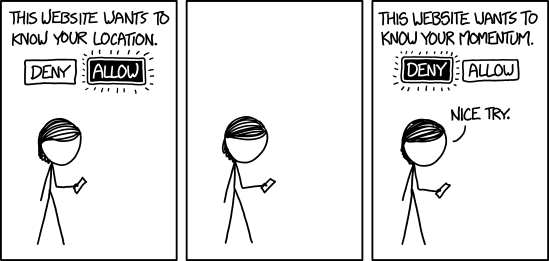
\includegraphics[width=0.8\hsize]{images/xkcd-location-sharing.png}
\caption{XKCD Comic zur Heisenberg Unsch"arfe. Die Benutzerin stellt sicher,
dass die Heisenbergsche Unsch"arferelation nicht verletzt wird. Man kann nicht
sowohl den Ort als auch den Impuls wissen.
\label{skript:heisenberg:xkcd}}
\end{figure}
Im Kapitel~\ref{chapter:drehimpuls} werden wir ein weiteres Paar
von Operatoren wie Ort und Impuls kennen lernen.
Dort untersuchen wir die Komponente $L_3$ des Drehimpulses in $z$-Richtung.
Die dazugeh"orige Ortskoordinaten ist in Kugelkoordinaten die geographische 
L"ange $\varphi$ des Teilchens, welche durch eine Observable mit Operator
$\Phi$ festgestellt werden kann.
In Kugelkoordinaten hat $L_3$ die Form
\[
L_3=\frac{\hbar}{i}\frac{\partial}{\partial\varphi}.
\]
Die Vertauschungsrelationen f"ur $\Phi$ und $L_3$ sind
\[
[\Phi,L_3]=\frac{\hbar}{i}\operatorname{id},
\]
das entspricht den Vertauschungsrelationen von $X$ und $P$.
Zu $\Phi$ und $L_3$ geh"ort nach Satz~\ref{skript:robertson-schroedinger-unschaerfe}
die Unsch"arferelation
\[
\Delta\varphi\cdot\Delta l_3 \ge \frac{\hbar}2,
\]
man kann also den Drehimpuls und die Richtung $\varphi$ nicht gleichzeitig
beliebig genau kennen.
Dies erkl"art den Mouse-Over-Text des Comics in
Abbildung~\ref{skript:heisenberg:xkcd}:
\begin{quote}
Our phones must have great angular momentum sensors because
the compasses really suck.
\end{quote}

\subsection{Unsch"arfe von Energie und Zeit}
In unserem Formalismus hat die Zeit-Koordinate eine ausgezeichnete
Bedeutung, die Schr"odingergleichung beschreibt die Entwicklung
der Zust"ande in der Ortsdarstellung.
Dies hat zur Folge, das wir eine Unsch"arferelation zwischen Energie
und Zeit nicht aus der Robertson-Schr"odinger-Unsch"arferelation
(\ref{skript:uncertainty}) herleiten k"onnen.

Dazu br"auchten wir eine Theorie, welche Orts- und Zeitkoordinaten
gleichwertig behandelt.
Eine solche Theorie ist die spezielle Relativit"atstheorie, welche
zeigt, wie Raum und Zeit untrennbar in einer vierdimensionalen
Raumzeit miteinander verbunden sind.

F"ur einen Spezialfall kann man eine Unsch"arferelation zwischen
Energie und Zeit finden.
Betrachten wir dazu ein Photon mit Energie $E=h\nu$.
Schon die klassische Elektrodynamik erkl"art das Ph"anomen des
Strahlungsdrucks, welches auch schon von Raumfahrzeugen ausgenutzt
werden ist, um durch das Sonnensystem zu `segeln'.
Strahlungsdruck bedeutet, dass Photonen Impuls $p=E/c$ transportieren
und "ubertragen.
Da alle Photonen gleich schnell sind, n"amlich $c$, ist die
Positionsunsch"arfe $\Delta x$ eines Photons im Wesentlichen die
Zeitunsch"arfe der Messung $\Delta t$.
Die Heisenbergsche Unsch"arferelation wird daher
\[
\frac{\hbar}2\le \Delta x\cdot\Delta p=c\Delta t\cdot \frac{\Delta E}{c}=
\Delta t\cdot \Delta E.
\]
Die Unsch"arfe zwischen Zeit und Energie bedeutet, dass die
Energieerhaltung um den Betrag $\Delta E$ verletzt werden darf,
wenn auch nur f"ur kurze Zeit $\Delta t$.

\section*{"Ubungsaufgaben}
\rhead{"Ubungsaufgaben}
\begin{uebungsaufgaben}
\item
Betrachten Sie die beiden Teilchen im Einstein-Podolsky-Rosen Experiment
mit Ortsoperatoren $X_i$ und Impulsoperatorn $P_i$ mit $i=1,2$.
F"ur diese Operatoren gelten die Vertauschungsrelationen
$[X_i,P_i]=-i\hbar\operatorname{id}$, und wir k"onnen nicht
den Ort und den Impuls eines der Teilchens gleichzeig wissen.
Mit der experimentellen Vorschrift von Einstein, Podolsky und Rosen
bestimmt man nicht $X_1$ und $X_2$, sondern
die Differenz $X=X_1-X_2$, denn man kann nicht die Position des
Ausgangssystems messen, ohne es zu ver"andern. Ebenso kann man nicht
den Impuls eines Teilchens, sondern nur den Gesamtimpuls $P=P_1-P_2$ 
bestimmen. Zeigen Sie, dass man diese beiden Gr"ossen tats"achlich
beide beliebig genau wissen kann, dass das klassische Einsten-Podolsky-Rosen
Experiment also keinen Widerspruch zur Unsch"arferelation darstellt.

\begin{loesung}
Man muss den Kommutator $[X,P]$ bestimmen:
\begin{align*}
[X,P]
&=
[X_1-X_2,P_1-P_2]
=
\underbrace{[X_1,P_1]}_{i\hbar\operatorname{id}}
-\underbrace{[X_2,P_1]}_{=0}
-\underbrace{[X_1,P_2]}_{=0}
-\underbrace{[X_2,P_2]}_{i\hbar\operatorname{id}}
=
i\hbar\operatorname{id}
-i\hbar\operatorname{id}
=0
\end{align*}
Die beiden Operatoren vertauschen, also k"onnen sie tats"achlich gleichzeit
beliebig genau bestimmt sein.
\end{loesung}



\item
Kann man Impuls und Energie eines Teilchens beliebig genau wissen?
Wenn ja, formulieren Sie eine Unsch"arferelation.

\begin{loesung}
Man kann Impuls und Energie eines Teilchens genau dann bleibig genau
wissen, wenn die zugeh"origen Operatoren $P$ und $H$ vertauschen.
Also berechnen wir den Kommutator:
\begin{align*}
[P,H]
&=
\biggl[P,\frac1{2m}P^2+V\biggr]
=
[P,V].
\end{align*}
Wir k"onnen daraus schon mal ablesen, dass f"ur ein freies Teilchen,
also f"ur $V=0$, die beiden Operatoren tats"achlich vertauschbar sind,
wir k"onnen also tats"achlich Impuls und Energie gleichzeitig 
beliebig genau kennen.

Wenn $V\ne 0$ ist, m"ussen wir den Kommutator von $P$ mit $V$
bestimmen:
\begin{align*}
[P,V]
&=
\biggl[\frac{\hbar}{i}\frac{\partial}{\partial x}, V\biggr]
=
\frac{\hbar}{i}
\biggl(
\frac{\partial}{\partial x}
V
-
V
\frac{\partial}{\partial x}
\biggr)
=
\frac{\hbar}{i}
\biggl(
\frac{\partial V}{\partial x}
+
V
\frac{\partial}{\partial x}
-
V
\frac{\partial}{\partial x}
\biggr)
=
\frac{\hbar}{i}
\frac{\partial V}{\partial x}.
\end{align*}
Die zugeh"orige Unsch"arferelation ist
\[
\Delta p\cdot \Delta E
=
\frac{\hbar}{2m}\biggl\langle \frac{\partial V}{\partial x}\biggr\rangle.
\]
F"ur schwere Teilchen, also zum Beispiel f"ur makroskopische K"orper ist
die Unsch"arfe nicht wahrnehmbar.
Die Unsch"arfe ist also umso gr"osser, je gr"osser die Ableitung des
Potentials ist.
Physikalisch kann man dies damit erkl"aren, dass es bei bekanntem Impuls
keine scharfe Position eines Teilchens gibt, die Energie wird also an
verschiedenen Orten gemessen, wo verschiedene potentielle Energien 
gemessen werden.
Die Ableitung des Potentials ist aber die Kraft, die auf ein Teilchen wirkt.
Die Unsch"arfe ist also umso gr"osser, je gr"osser die Kr"afte sind, die
auf das Teilchen wirken.
\end{loesung}


\item
Kann man Energie und Position eines Teilchens beliebig genau wissen?
Wenn nicht, formulieren Sie eine entsprechende Unsch"arferelation.

\begin{loesung}
Die Energie eines Teilchens wird durch die Observable $H$, den
Hamilton-Operator gegeben.
Die Position wird hingegen durch den Operator $X$ der Position
gegeben.
Man kann beide beleibig genau wissen, d.~h.~es gibt gemeinsame
Eigenzust"ande von $H$ und $X$, wenn die beiden Operatoren vertauschen.
Wir berechnen daher den Kommutator von $X$ und $H$:
\begin{align*}
[X,H]
&=
\biggl[X,\frac1{2m}P^2\biggr]
=
\frac1{2m}[X,P^2]
=
\frac1{2m}(XPP-PPX)
=
\frac1{2m}(XPP-PXP+PXP-PPX)
\\
&=
\frac1{2m}([X,P]P+P[X,P])
=
-\frac{\hbar}{im} P
\end{align*}
Die zugeh"orige Unsch"arferelation ist
\[
\Delta E\cdot \Delta x\ge \frac{\hbar}{2m}\langle P\rangle
=
\frac{\hbar}{2}\langle v\rangle.
\]
Die Unsch"arfe h"angt also vom Impuls eines Teilchens ab, je gr"osser
der Impuls, desto gr"osser auch die Unsch"arfe.
\end{loesung}


\end{uebungsaufgaben}
